\documentclass{article}
\usepackage{ismir,amsmath,cite}
\usepackage{amssymb}
\usepackage{graphicx}
\usepackage{color}
\usepackage{framed}
\usepackage{booktabs}
\usepackage[letterspace=-22]{microtype}

\title{\textls{Large-Scale Content-Based Matching of MIDI and Audio Files}}

\oneauthor
  {Colin Raffel, Daniel P. W. Ellis} {LabROSA, Department of Electrical Engineering \\ Columbia University, New York, NY \\ \texttt{\{craffel,dpwe\}@ee.columbia.edu}}


\begin{document}

\maketitle

\begin{abstract}
  MIDI files, when paired with corresponding audio recordings, can be used as ground truth for many music information retrieval tasks.
  We present a system which can efficiently match and align MIDI files to entries in a large corpus of audio content based solely on content, i.e., without using any metadata.
  The core of our approach is a convolutional network-based cross-modality hashing scheme which transforms feature matrices into sequences of vectors in a common Hamming space.
  Once represented in this way, we can efficiently perform large-scale dynamic time warping searches to match MIDI data to audio recordings.
  We evaluate our approach on the task of matching a huge corpus of MIDI files to the Million Song Dataset.
\end{abstract}

\section{Training Data for MIR}\label{sec:introduction}

Central to the task of content-based Music Information Retrieval (MIR) is the curation of ground-truth data for tasks of interest (e.g. timestamped chord labels for automatic chord estimation, beat positions for beat tracking, prominent melody time series for melody extraction, etc.).
The quantity and quality of this ground-truth is often instrumental in the success of MIR systems which utilize it as training data.
Creating appropriate labels for a recording of a given song by hand typically requires person-hours on the order of the duration of the data, and so training data availability is a frequent bottleneck in content-based MIR tasks.

MIDI files that are time-aligned to matching audio can provide ground-truth information  \cite{ewert2012towards, turetsky2003ground} and can be utilized in score-informed source separation systems \cite{ewert2014score, ganseman2010source}.
A MIDI file can serve as a timed sequence of note annotations (a ``piano roll'').
It is much easier to estimate information such as beat locations, chord labels, or predominant melody from these representations than from an audio signal.
A number of tools have been developed for inferring this kind of information from MIDI files \cite{eerola2004mir,mckay2006jsymbolic,cuthbert2010music21,raffel2014pretty_midi}.


Halevy et al. \cite{halevy2009unreasonable} argue that some of the biggest successes in machine learning came about because ``...a large training set of the input-output behavior that we seek to automate is available to us in the wild.''
The motivation behind this project is that MIDI files fit this description.
Through a large-scale web scrape, we obtained 455,333 MIDI files, 140,910 of which were unique -- orders of magnitude larger than any available dataset of aligned transcriptions.
This proliferation of data is likely due to the fact that MIDI files are typically a few kilobytes in size and were therefore a popular format for distributing and storing music recordings when hard drives had only megabytes of storage.

%\subsection{Wrangling MIDI files}

The mere existence of a large collection of MIDI data is not enough:  In order to use MIDI files as ground truth, they need to be both matched (paired with a corresponding audio recording) and aligned (adjusted so that the timing of the events in the file match the audio).
Alignment has been studied extensively  \cite{ewert2012towards, turetsky2003ground}, but prior work typically assumes that the MIDI and audio have been correctly matched.
Given large corpora of audio and MIDI files, the task of matching entries of each type may seem to be a simple matter of fuzzy text matching of the files' metadata.
However, MIDI files almost never contain structured metadata, and as a result the best-case scenario is that the artist and song title are included in the file or directory name.
While we found some examples of this in our collection of scraped MIDI files, the vast majority of the files had effectively no metadata information.
Figure \ref{fig:midi-names} shows a random sampling of directory and filenames from our collection.

\begin{figure}
  \begin{framed}
    \scriptsize
    \tt
    J/Jerseygi.mid

    V/VARIA18O.MID

    Carpenters/WeveOnly.mid

    2009 MIDI/handy\char`_man1-D105.mid

    G/Garotos Modernos - Bailanta De Fronteira.mid

    Various Artists/REWINDNAS.MID

    GoldenEarring/Twilight\char`_Zone.mid

    Sure.Polyphone.Midi/Poly 2268.mid

    d/danza3.mid

    100\%sure.polyphone.midi/Fresh.mid

    rogers\char`_kenny/medley.mid

    2009 MIDI/looking\char`_out\char`_my\char`_backdoor3-Bb192.mid
  \end{framed}

  \caption{Random sampling of 12 MIDI filenames and their parent directories from our corpus of 455,333 MIDI files scraped from the Internet.}
  \label{fig:midi-names}
\end{figure}

Since the goal of matching MIDI and audio files is to find pairs that have \textit{content} in common, we can in principle identify matches regardless of metadata availability or accuracy.
However, comparing content is more complicated and more expensive than a fuzzy text match.
Since $NM$ comparisons are required to match a MIDI dataset of size $N$ to an audio file dataset of size $M$, matching large collections is practical only when the individual comparisons can be made very fast.
Thus, the key aspect of our work is a {\em highly-efficient} scheme to match the content of MIDI and audio files.
Our system learns a cross-modality hashing which converts both MIDI and audio content vectors to a common Hamming (binary) space in which the ``local match'' operation at the core of dynamic time warping (DTW) reduces to a very fast table lookup.
As described below, this allows us to match a single MIDI file to a huge collection of audio files in minutes rather than hours.

The idea of using DTW distance to match MIDI files to audio recordings is not new.
For example, in \cite{hu2003polyphonic}, MIDI-audio matching is done by finding the minimal DTW distance between all pairs of chromagrams of (synthesized) MIDI and audio files.
Our approach differs in a few key ways: First, instead of using chromagrams (a hand-designed representation), we learn a common representation for MIDI and audio data.
Second, our datasets are many orders of magnitude larger (hundreds of thousands vs.\ hundreds of files), which necessitates a much more efficient approach.
Specifically, by mapping to a Hamming space we greatly speed up distance matrix calculation and we receive quad\-rat\-ic speed gains by implicitly downsampling the audio and MIDI feature sequences as part of our learned feature mapping.

In the following section, we detail the dataset of MIDI files we scraped from the Internet and describe how we prepared a subset for training our hasher.
Our cross-modality hashing model is described in Section \ref{sec:hashing}.
Finally, in section \ref{sec:msd} we evaluate our system's performance on the task of matching files from our MIDI dataset to entries in the Million Song Dataset \cite{bertin2011million}.

\section{Preparing Data}
\label{sec:dataset}

Our project began with a large-scale scrape of MIDI files from the Internet.
We obtained 455,333 files, of which 140,910 were found to have unique MD5 checksums.
The great majority of these files had little or no metadata information.
The goal of the present work is to develop an efficient way to match this corpus against the Million Song Dataset (MSD), or, more specifically, to the short preview audio recordings provided by 7digital \cite{schindler2012facilitating}.

For evaluation, we need a collection of ground-truth MIDI-audio pairs which are correctly matched.
Our approach can then be judged based on how accurately it is able to recover these pairings using the content of the audio and MIDI files alone.
To develop our cross-modality hashing scheme, we further require a collection of {\em aligned} MIDI and audio files, to supply the matching pairs of feature vectors from each domain that will be used to train our model for hashing MIDI and audio features to a common Hamming space (described in Section \ref{sec:hashing}).
Given matched audio and MIDI files, existing alignment techniques can be used to create this training data; however, we must exclude incorrect matches and failed alignments.
Even at the scale of this reduced set of training data, manual alignment verification is impractical, so we developed an improved alignment quality score which we describe in Section \ref{sec:score}.

\subsection{Metadata matching}

To obtain a collection of MIDI-audio pairs, we first separated a subset of MIDI files for which the directory name corresponded to the song's artist and the filename gave the song's title.
The resulting metadata needed additional canonicalization; for example, ``The Beatles'', ``Beatles, The'', ``Beatles'', and ``The Beatles John Paul Ringo George'' all appeared as artists.
To normalize these issues, we applied some manual text processing and resolved the artists and song titles against the Freebase \cite{bollacker2008freebase} and Echo Nest\footnote{\texttt{http://developer.echonest.com/docs/v4}} databases.
This resulted in a collection of 17,243 MIDI files for 10,060 unique songs, which we will refer to as the ``clean MIDI subset''.

We will leverage the clean MIDI subset in two ways: First, to obtain ground-truth pairings of MSD/MIDI matches, and second, to create training data for our hashing scheme.  
The training data does not need to be restricted to the MSD, and using other sources to increase the training set size will likely improve our hashing performance, so we combined the MSD with three benchmark audio collections: CAL500 \cite{turnbull2007towards}, CAL10k \cite{tingle2010exploring}, and uspop2002 \cite{berenzweig2004large}.
To match these datasets to the clean MIDI subset, we used the Python search engine library \texttt{whoosh}\footnote{\texttt{https://github.com/dokipen/whoosh}} to perform a fuzzy matching of their metadata.
This resulted in 26,311 audio/MIDI file pairs corresponding to 5,243 unique songs.

\subsection{Aligning audio to synthesized MIDI}
\label{sec:alignment}

Fuzzy metadata matching is not enough to ensure that we have MIDI and audio files with matching content: For instance, the metadata could be incorrect, the fuzzy text match could have failed, the MIDI could be a poor transcription (e.g., missing instruments or sections), and/or the MIDI and audio data could correspond to different versions of the song.
Since we will use DTW to align the audio content to an audio resynthesis of the MIDI content \cite{turetsky2003ground, hu2003polyphonic,ewert2012towards}, we could potentially use the overall match cost -- the quantity minimized by DTW -- as an indicator of valid matches, since unrelated MIDI and audio pairs will likely result in a high optimal match cost.  (An overview of DTW and its application to music can be found in \cite{muller2007information}.)

Unfortunately, the calibration of this raw match cost ``confidence score'' is typically not comparable between different alignments.  
Our application, however, requires a DTW confidence score that can reliably decide when an audio/MIDI file pairing is valid for use as training data for our hashing model.
Our best results came from the following system for aligning a single MIDI/audio file pair:
First, we synthesize the MIDI data using \texttt{fluidsynth}.\footnote{\texttt{http://www.fluidsynth.org}}
We then estimate the MIDI beat locations using the MIDI file's tempo change information and the method described in \cite{raffel2014pretty_midi}.
To circumvent the common issue where the beat is tracked one-half beat out of phase, we double the BPM until it is at least 240.
We compute\footnote{All audio analysis was accomplished with \texttt{librosa} \cite{mcfee2014librosa}.} beat locations for the audio signal with the constraint that the BPM should remain close to the global MIDI tempo.
We then compute log-amplitude beat-synchronous constant-Q transforms (CQTs) of audio and synthesized MIDI data with semitone frequency spacing and a frequency range from C3 (65.4 Hz) to C7 (1046.5 Hz).
The resulting feature matrices are then of dimensionality $N \times D$ and $M \times D$ where $N$ and $M$ are the resulting number of beats in the MIDI and audio recordings respectively and $D$ is $48$ (the number of semitones between C3 and C7).
Example CQTs computed from a 7digital preview clip and from a synthesized MIDI file can be seen in Figure \ref{fig:simdtw}(a) and \ref{fig:simdtw}(b) respectively.

\begin{figure*}
  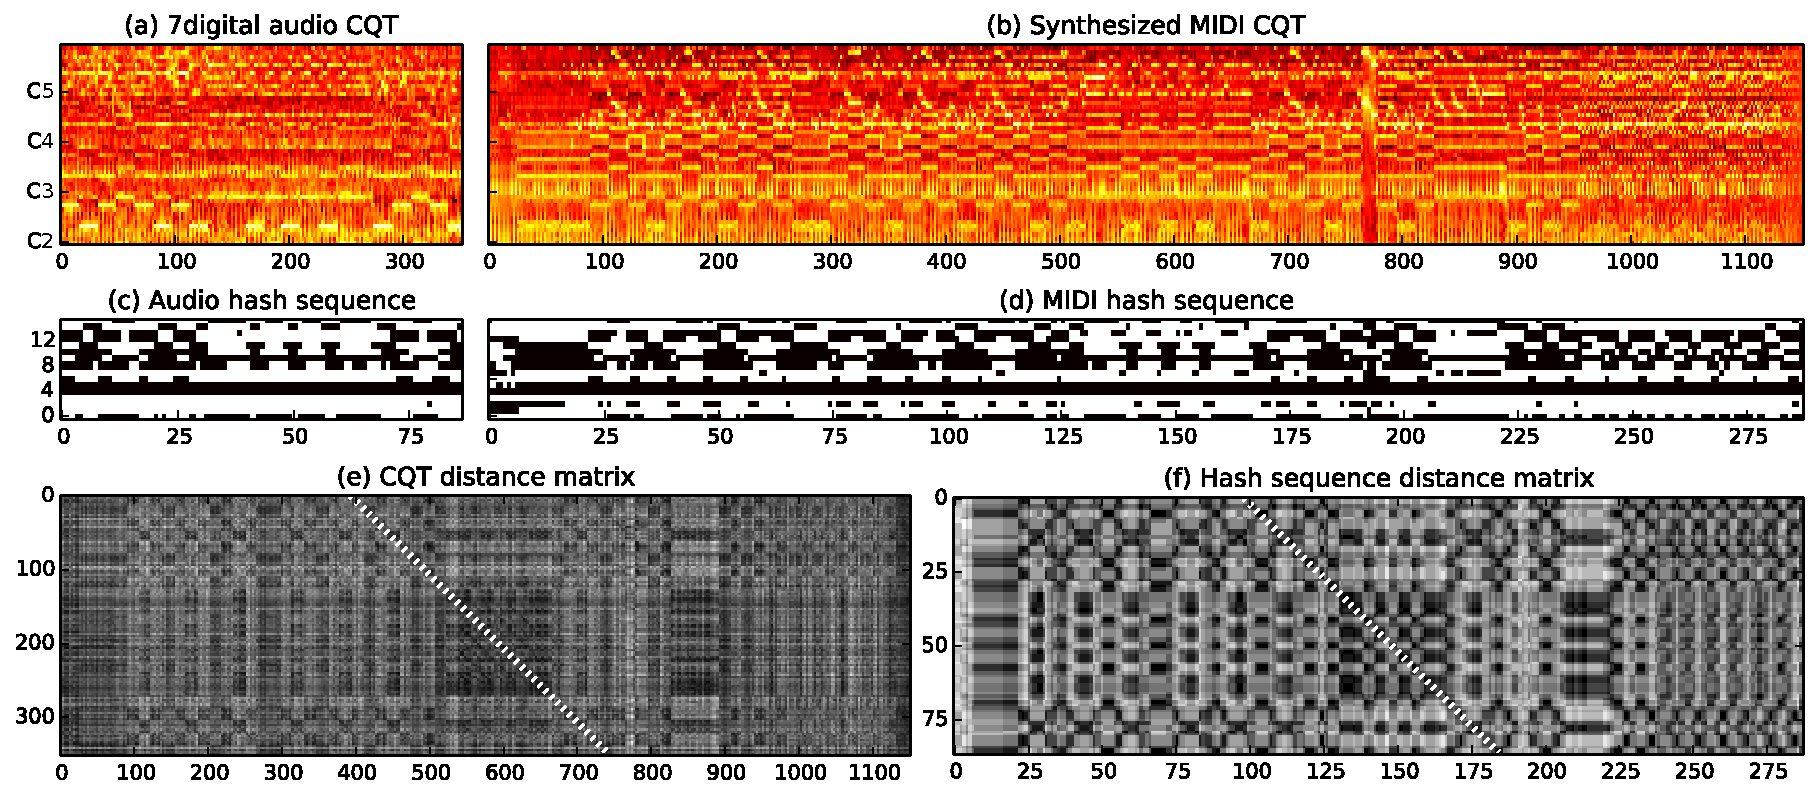
\includegraphics[width=\textwidth]{sims_and_dtws.pdf}
  \caption{Audio and hash-based features and alignment for Billy Idol - ``Dancing With Myself'' (MSD track ID \texttt{TRCZQLG128F427296A}).
           (a) Normalized constant-Q transform of 7digital preview clip, with semitones on the vertical axis and beats on the horizontal axis.
	   (b) Normalized CQT for synthesized MIDI file.
	   (c) Hash bitvector sequence for 7digital preview clip, with pooled beat indices and Hamming space dimension on the horizontal and vertical axes respectively.
	   (d) Hash sequence for synthesized MIDI.
	   (e) Distance matrix and DTW path (displayed as a white dotted line) for CQTs.  Darker cells indicate smaller distances.
	   (f) Distance matrix and DTW path for hash sequences.}
  \label{fig:simdtw}
\end{figure*}

We then use DTW to find the lowest-cost path through a full pairwise cosine distance matrix $S \in \mathbb{R}^{N \times M}$ of the MIDI and audio CQTs.
This path can be represented as two sequences $p, q \in \mathbb{R}^L$ of indices from each sequence such that $p[i] = n, q[i] = m$ implies that the $n$th MIDI beat should be aligned to the $m$th audio beat.
Traditional DTW constrains this path to include the start and end of each sequence, i.e. $p[1] = q[1] = 1$ and $p[L] = N; q[L] = M$.
However, the MSD audio consists of cropped preview clips from 7digital, while MIDI files are generally transcriptions of the entire song.
We therefore modify this constraint so that either $gN \le p[L] \le N$ or $gM \le q[L] \le M$; $g$ is a parameter which provides a small amount of additional tolerance and is normally close to $1$.
We employ an additive penalty $\phi$ for ``non-diagonal moves'' (i.e. path entries where either $p[i] = p[i + 1]$ or $q[i] = q[i + 1]$) which, in our setting, is set to approximate a typical distance value in $S$.
The combined use of $g$ and $\phi$ typically results in paths where both $p[1]$ and $q[1]$ are close to $1$, so no further path constraints are needed.
For synthesized MIDI-to-audio alignment, we used $g = .95$ and set $\phi$ to the 90th percentile of all the values in $S$.
The cosine distance matrix and the lowest-cost DTW path for the CQTs shown in Figure \ref{fig:simdtw}(a) and \ref{fig:simdtw}(b) can be seen in Figure \ref{fig:simdtw}(e).

\subsection{DTW cost as confidence score}
\label{sec:score}

The cost of a DTW path $p, q$ through $S$ is calculated by the sum of the distances between the aligned entries of each sequence:
$$
c = \sum_{i = 1}^L S[p[i], q[i]] + T(p[i] - p[i-1], q[i] - q[i-1])
$$
where the transition cost term $T(u,v) = 0$ if $u$ and $v$ are 1, otherwise $T(u, v) = \phi$.
As discussed in \cite{hu2003polyphonic}, this cost is not comparable between different alignments for two main reasons: Firstly, the path length can vary greatly across MIDI/audio file pairs depending on $N$ and $M$.
We therefore prefer a per-step {\em mean} distance, where we divide $c$ by $L$.
Secondly, various factors irrelevant to alignment such as differences in production and instrumentation can effect a global shift on the values of $S$, even when its local variations still reveal the correct alignment.  
This can be mitigated by normalizing the DTW cost by the mean value of the submatrix of $S$ containing the DTW path:
$$
\mathcal{B} = \sum_{i = \min(p)}^{\max(p)} \sum_{j = \min(q)}^{\max(q)} S[i, j] 
$$
We combine the above to obtain a modified DTW cost $\hat{c}$:
$$
\hat{c} = \frac{c}{L \mathcal{B}}
$$

To estimate the largest value of $\hat{c}$ for acceptable alignments, we manually auditioned 125 alignments and recorded whether the audio and MIDI were well-synchronized for their entire duration, our criterion for acceptance.
This ground-truth supported a receiver operating characteristic (ROC) for $\hat{c}$ with an AUC score of $0.986$, indicating a highly reliable confidence metric.
A threshold of $0.78$ allowed zero false accepts on this set while only falsely discarding 15 well-aligned pairs.
Retaining all alignments with costs better (lower) than this threshold resulted in 10,035 successful alignments.

Recall that these matched and aligned pairs serve two purposes: They provide training data for our hashing model; and we also use them to evaluate the entire content-based matching system.
For a fair evaluation, we exclude items used in training from the evaluation, thus we split the successful alignments into three parts: 50\% to use as training data, $25\%$ as a ``development set'' to tune the content-based matching system, and the remaining $25\%$ to use for final evaluation of our system.
Care was taken to split based on \textit{songs}, rather than by entry (since some songs appear multiple times).

\section{Cross-Modality Hashing of MIDI and Audio Data}
\label{sec:hashing}

We now arrive at the central part of our work, the scheme for hashing both audio and MIDI data to a  common simple representation to allow very fast computation of the distance matrix $S$ needed for DTW alignment.
In principle, given the confidence score of the previous section, to find audio content that matches a given MIDI file, all we need to do is perform alignment against every possible candidate audio file and choose the audio file with the lowest score.
To maximize the chances of finding a match, we need to use a large and comprehensive pool of audio files.
We use the 994,960 7digital preview clips corresponding to the Million Song Dataset, which consist of (typically) 30 second portions of recordings from the largest standard research corpus of popular music \cite{schindler2012facilitating}.
A complete search for matches could thus involve 994,960 alignments for each of our 140,910 MIDI files.

The CQT-to-CQT approach of section \ref{sec:alignment} cannot feasibly achieve this.
The median number of beats in our MIDI files is 1218, and for the 7digital preview clips it is 186.
Computing the cosine distance matrix $S$ of this size (for $D=48$ dimension CQT features) using the highly optimized C++ code from \texttt{scipy} \cite{jones2014scipy} takes on average 9.82 milliseconds on an Intel Core i7-4930k processor.
When implemented using the LLVM just-in-time compiler Python module \texttt{numba},\footnote{\texttt{http://numba.pydata.org/}} the DTW cost calculation described above takes on average 892 microseconds on the same processor.
Matching a \textit{single} MIDI file to the MSD using this approach would thus take just under three hours; matching our entire 140,910 MIDI file collection to the MSD would take years.
Clearly, a more efficient approach is necessary.

Calculating the distance matrix and the DTW cost are both $\mathcal{O}(NM)$ in complexity; the distance matrix calculation is about 10 times slower presumably because it involves $D$ multiply-accumulate operations to compute the inner product for each point.
Calculating the distance between feature vectors is therefore the bottleneck in our system, so any reduction in the number of feature vectors (i.e., beats) in each sequence will give quadratic speed gains for both DTW and distance matrix calculations.

Motivated by these issues, we propose a system which learns a common, reduced representation for the audio and MIDI features in a Hamming space.
By replacing constant-Q spectra with bitvectors, we replace the expensive inner product computation by an exclusive-or operation followed by simple table lookup: The exclusive-or of two bitvectors $a$ and $b$ will yield a bitvector consisting of $1$s where $a$ and $b$ differ and $0$s elsewhere, and the number of $1$s in all bitvectors of length $D$ can be precomputed and stored in a table of size $2^D$.  
In the course of computing our Hamming space representation, we also implicitly downsample the sequences over time, which provides speedups for both distance matrix and DTW calculation.
Our approach has the additional potential benefit of {\em learning} the most effective representation for comparing audio and MIDI constant-Q spectra, rather than assuming the cosine distance of CQT vectors is suitable.

\subsection{Hashing with convolutional networks}

Our hashing model is based on the Siamese network architecture proposed in \cite{masci2014multimodal}.
Given feature vectors $\{x\}$ and $\{y\}$ from two modalities, and a set of pairs $\mathcal{P}$ such that $(x, y) \in \mathcal{P}$ indicates that $x$ and $y$ are considered ``similar'', and a second set $\mathcal{N}$ consisting of ``dissimilar'' pairs, a nonlinear mapping is learned from each modality to a common Hamming space such that similar and dissimilar feature vectors are respectively mapped to bitvectors with small and large Hamming distances.
A straightforward objective function which can be minimized to find an appropriate mapping is
\begin{align*}
\mathcal{L} &= \frac{1}{|\mathcal{P}|} \sum_{(x, y) \in \mathcal{P}} \| f(x) - g(y) \|_2^2\\
& - \frac{\alpha}{|\mathcal{N}|} \sum_{(x, y) \in \mathcal{N}} \max(0, m - \|f(x) - g(y) \|_2)^2
\end{align*}
where $f$ and $g$ are the nonlinear mappings for each modality, $\alpha$ is a parameter to control the importance of separating dissimilar items, and $m$ is a target separation of dissimilar pairs.

The task is then to optimize the nonlinear mappings $f$ and $g$ with respect to $\mathcal{L}$.
In \cite{masci2014multimodal} the mappings are implemented as multilayer nonlinear networks.
In the present work, we will use convolutional networks due to their ability to exploit invariances in the input feature representation; CQTs contain invariances in both the time and frequency axes, so convolutional networks are particularly well-suited for our task.
Our two feature modalities are CQTs from synthesized MIDI files and audio files.
We assemble the set of ``similar'' cross-modality pairs $\mathcal{P}$ by taking the CQT frames from individual aligned beats in our training set.
The choice of $\mathcal{N}$ is less obvious, but randomly choosing CQT spectra from non-aligned beats in our collection achieved satisfactory results.

\subsection{System specifics}

Training the hashing model involves presenting training examples and backpropagating the gradient of $\mathcal{L}$ through the model parameters.
We held out 10\% of the training set described in Section \ref{sec:dataset} as a validation set, not used in training the networks.
We z-scored the remaining 90\% across feature dimensions and re-used the means and standard deviations from this set to z-score the validation set.

For efficiency, we used minibatches of training examples; each minibatch consisted of 50 sequences obtained by choosing a random offset for each training sequence pair and cropping out the next 100 beats.  
For $\mathcal{N}$, we simply presented the network with subsequences chosen at random from different songs. 
Each time the network had iterated over minibatches from the entire training set (one epoch), we repeated the random sampling process. 
For optimization, we used RMSProp, a recently-proposed stochastic optimization technique \cite{tieleman2012lecture}.
After each 100 minibatches, we computed the loss $\mathcal{L}$ on the validation set.
If the validation loss was less than $99\%$ of the previous lowest, we trained for 1000 more iterations (minibatches).

While the validation loss is a reasonable indicator of network performance, its scale will vary depending on the $\alpha$ and $m$ regularization hyperparameters.
To obtain a more consistent metric, we also computed the distribution of distances between the hash vectors produced by the network for the pairs in $\mathcal{P}$ and those in $\mathcal{N}$.
To directly measure network performance, we used the Bhattacharya distance \cite{bhattacharyya1943measure} to compute the separation of these distributions.

In each modality, the hashing networks have the same architecture: A series of alternating convolutional and pooling layers followed by a series of fully-connected layers.
All layers except the last use rectifier nonlinearities; as in \cite{masci2014multimodal}, the output layer uses a hyperbolic tangent.
This choice allows us to obtain binary hash vectors by testing whether each output unit is greater or less than zero.
We chose 16 bits for our Hamming space, since 16 bit values are efficiently manipulated as short unsigned integers.
The first convolutional layer has 16 filters each of size 5 beats by 12 semitones, which gives our network some temporal context and octave invariance.
As advocated by \cite{simonyan2014very}, all subsequent convolutional layers had $2^{n + 3}$ 3$\times$3 filters, where $n$ is the depth of the layer.
All pooling layers performed max-pooling, with a pooling size of 2$\times$2.
Finally, as suggested in \cite{he2015delving}, we initialized all weights with normally-distributed random variables with mean of zero and a standard deviation of $\sqrt{2/n_{in}}$, where $n_{in}$ is the number of inputs to each layer.
Our model was implemented using \texttt{theano} \cite{bastien2012theano} and \texttt{lasagne}.\footnote{\texttt{https://github.com/Lasagne/Lasagne}}

To ensure good performance, we optimized all model hyperparameters using Whetlab,\footnote{Between submission and acceptance of this paper, Whetlab announced it would be ending its service.  For posterity, the results of our hyperparameter search are available at \texttt{http://bit.ly/hash-param-search}.} a web API which implements black-box Bayesian optimization \cite{snoek2012practical}.
We used Whetlab to optimize the number of convolutional/pooling layers, the number and size of the fully-connected layers, the RMSProp learning rate and decay parameters, and the $\alpha$ and $m$ regularization parameters of $\mathcal{L}$.
As a hyperparameter optimization objective, we used the Bhattacharyya distance as described above.
The best performing network found by Whetlab had 2 convolutional layers, 2 ``hidden'' fully-connected layers with 2048 units in addition to a fully-connected output layer, a learning rate of .001 with an RMSProp decay parameter of .65, $\alpha = .5$, and $m = 4$.
This hyperparameter configuration yielded the output hash distance distributions for $\mathcal{P}$ and $\mathcal{N}$ shown in Figure \ref{fig:distances}, for a Bhattacharyya separation of $0.488$.

\begin{figure}
  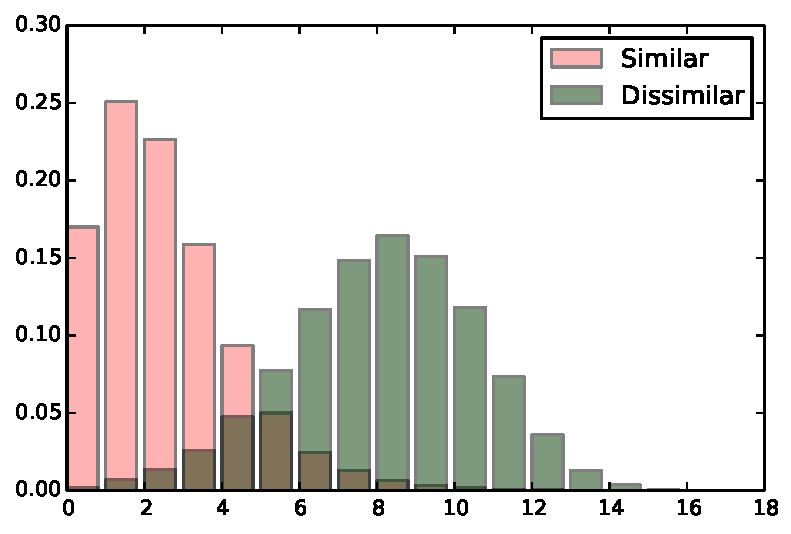
\includegraphics[width=\columnwidth]{hash_distributions.pdf}
  \caption{Output hash distance distributions for our best-performing network.}
  \label{fig:distances}
\end{figure}

\section{Matching MIDI Files to the MSD}
\label{sec:msd}

After training our hashing system as described above, the process of matching MIDI collections to the MSD proceeds as follows:
First, we precompute hash sequences for every 7digital preview clip and every MIDI file in the clean MIDI subset.
Note that in this setting we are not computing feature sequences for known MIDI/audio pairs, so we cannot force the audio's beat tracking tempo to be the same as the MIDI's; instead, we estimate their tempos independently.
Then, we compute the DTW cost as described in Section \ref{sec:alignment} between every audio and MIDI hash sequence.

We tuned the parameters of the DTW cost calculation to optimize results over our ``development'' set of successfully aligned MIDI/MSD pairs.
We found it beneficial to use a smaller value of $g = 0.9$.
Using a fixed value for the non-diagonal move penalty avoids the percentile calculation, so we chose $\phi = 4$.
Finally, we found that normalizing by the average distance value $\mathcal{B}$ did not help, so we skipped this step.

\subsection{Results}

Bitvector sequences for the CQTs shown in Figure \ref{fig:simdtw}(a) and \ref{fig:simdtw}(b) can be seen in \ref{fig:simdtw}(c) and \ref{fig:simdtw}(d) respectively.
Note that because our networks contain two downsample-by-2 pooling layers, the number of bitvectors is $\frac{1}{4}$ of the number of constant-Q spectra for each sequence.
The Hamming distance matrix and lowest-cost DTW path for the hash sequences are shown in Figure \ref{fig:simdtw}(f).
In this example, we see the same structure as in the CQT-based cosine distance matrix of  \ref{fig:simdtw}(e), and the same DTW path was successfully obtained.

To evaluate our system using the known MIDI-audio pairs of our evaluation set, we rank MSD entries according to their hash sequence DTW distance to a given MIDI file, and determine the rank of the correct match for each MIDI file.
The correct item received a mean reciprocal rank of \textbf{$0.241$}, indicating that the correct matches tended to be ranked highly.  
Some intuition about the system performance is given by reporting the percentage of MIDI files in the test set where the correct match ranked below a certain threshold; this is shown for various thresholds in Table \ref{tab:rank-percentages}.

\begin{table}
  \begin{center}
    \begin{tabular}{@{}llllll@{}}
      \toprule
      \textbf{Rank} & 1 & 10 & 100 & 1000 & 10000 \\
      \textbf{Percent $\le$} & 15.2 & 41.6 & 62.8 & 82.7 & 95.9 \\
      \bottomrule
    \end{tabular}
  \end{center}
  \caption{Percentage of MIDI-MSD pairs whose hash sequences had a rank better than each threshold.}
  \label{tab:rank-percentages}
\end{table}

Studying Table \ref{tab:rank-percentages} reveals that we can't rely on the correct entry appearing as the top match among all the MSD tracks; the DTW distance for true matches only appears at rank 1 about 15.2\% of time.
Furthermore, for a significant portion of our MIDI files, the correct match did not rank in the top 1000.
This was usually caused by the MIDI file being beat tracked at a different tempo than the audio file, which inflated the DTW score.
For MIDI files where the true match ranked highly but not first, the top rank was often a different version (cover, remix, etc.) of the correct entry.
Finally, some degree of inaccuracy can be attributed to the fact that our hashing model is not perfect (as shown in Figure \ref{fig:distances}) and that the MSD is very large, containing many possible decoys. 
In a relatively small proportion of cases, the MIDI hash sequence ended up being very similar to many MSD hash sequences, pushing down the rank of the correct entry.

Given that we cannot reliably assume the top hit from hashing is the correct MSD entry, it is more realistic to look at our system as a pruning technique; that is, it can be used to discard MSD entries which we can be reasonably confident do not match a given MIDI file.
For example, Table \ref{tab:rank-percentages} tells us that we can use our system to compute the hash-based DTW score between a MIDI file and every entry in the MSD, then discard all but 1\% of the MSD and only risk discarding the correct match about 4.1\% of the time.
We could then perform the more precise DTW on the full CQT representations to find the best match in the remaining candidates.
Pruning methods are valuable only when they are substantially faster than performing the original computation; fortunately, our approach is orders of magnitude faster:
On the same Intel Core i7-4930k processor, for the median hash sequence lengths, calculating a Hamming distance matrix between hash sequences is about 400 times faster than computing the CQT cosine distance matrix (24.8 microseconds vs. 9.82 milliseconds) and computing the DTW score is about 9 times faster (106 microseconds vs. 892 microseconds).
These speedups can be attributed to the fact that computing a table lookup is much more efficient than computing the cosine distance between two vectors and that, thanks to downsampling, our hash-based distance matrices have $\frac{1}{16}$ of the entries of the CQT-based ones.
In summary, a straightforward way to describe the success of our system is to observe that we can, with high confidence, discard 99\% of the entries of the MSD by performing a calculation that takes about as much time as matching against 1\% of the MSD.

\section{Future work}

Despite our system's efficiency, we estimate that performing a full match of our 140,910 MIDI file collection against the MSD would still take a few weeks, assuming we are parallelizing the process on the 12-thread Intel i7-4930k.
There is therefore room for improving the efficiency of our technique.
One possibility would be to utilize some of the many pruning techniques which have been proposed for the general case of large-scale DTW search.
Unfortunately, most of these techniques rely on the assumption that the query sequence is of the same length or shorter than all the sequences in the database and so would need to be modified before being applied to our problem.
In terms of accuracy, as noted above most of our hash-match failures can be attributed to erroneous beat tracking.
With a better beat tracking system or with added robustness to this kind of error, we could improve the pruning ability of our approach.
We could also compare the accuracy of our system to a slower approach on a much smaller task to help pinpoint failure modes.
Even without these improvements, our proposed system will successfully provide orders of magnitude of speedup for our problem of resolving our huge MIDI collection against the MSD.
All the code used in this project is available online.\footnote{\texttt{http://github.com/craffel/midi-dataset}}

\section{Acknowledgements}

We would like to thank Zhengshan Shi and Hilary Mogul for preliminary work on this project and Eric J. Humphrey and Brian McFee for fruitful discussions.

\bibliography{refs}

\end{document}
